\chapter{Contraction Hierarchies, Hierarchical Hub Labelings}\label{chapter:ch}

Mit dem Aufkommen von Online-Kartendiensten in den 2000er-Jahren stieg der Bedarf an effizienten Algorithmen zur Berechnung kürzester Pfade in großen Netzwerken stark an.
Klassische Algorithmen wie der Dijkstra-Algorithmus sind für sehr große Graphen, wie etwa Straßennetze von ganzen Kontinenten, aufgrund ihrer hohen Zeitkomplexität nicht praktikabel.
Um diesem Problem zu begegnen, führten Geisberger et al. \cite{geisberger2008contraction} die Methode der \emph{Contraction Hierarchies} ein.
Diese nutzt ein ähnliches Konzept wie die in \autoref{graphs:strassengraphen} vorgestellte Idee der Wichtigkeit von Kanten und ermöglicht auf Straßengraphen einen Speedup um mehrere Größenordnungen.

Aufbauend auf diesem Ansatz entwickelten Abraham et al. \cite{abraham2011hub} einen Algorithmus, welcher aus der von \emph{Contraction Hierarchies} erzeugten Datenstruktur ein \emph{Hub Labeling} erzeugt.
Hub-Labeling-Anfragen sind effektiv Look-Ups und können noch einmal um Größenordnungen schneller als Contraction-Hierarchies-Anfragen sein.

In diesem Kapitel werden die theoretischen Grundlagen dieser Methoden detailliert erläutert.
Zudem wird in \autoref{chapter:kontraktion}  die Anwendbarkeit dieser Techniken auf Sichtbarkeitsgraphen untersucht.

\section{Contraction Hierarchies}

Die grundlegende Idee von Contraction Hierarchies besteht darin, die Berechnung von kürzesten Wegen in großen Graphen, wie Straßennetzen, durch eine effiziente \emph{Vorverarbeitung} zu beschleunigen.

Während der Vorverarbeitung werden die Knoten des Graphen in einer bestimmten Reihenfolge \emph{kontrahiert}, was bedeutet, dass sie entfernt werden.
Beim Entfernen eines Knotens werden \emph{Abkürzungen} zwischen seinen Nachbarn hinzugefügt, um sicherzustellen, dass die Abstände im übrigen Graphen erhalten bleiben.
Diese Abkürzungen ersetzen längere Pfade, die über den entfernten Knoten geführt hätten.

Durch die Kontraktion entsteht eine Hierarchie der Knoten, wobei \emph{weniger wichtige Knoten} zuerst kontrahiert werden.
Bei der eigentlichen Anfrage wird ein modifizierter bidirektionaler Dijkstra-Algorithmus verwendet, der die Hierarchie ausnutzt.
Die Suche beschränkt sich auf Kanten, die \emph{aufwärts} in der Hierarchie führen, was die Anzahl der während der Suche gesehenen Knoten stark reduzieren \emph{kann}.

\subsection{Knoten-Kontraktion}

Der Begriff Contraction Hierarchies leitet sich vom Konzept der Knoten-Kontraktion ab.

\begin{definition}[Knoten-Kontraktion]
  Sei $G = (V, E)$ ein Graph. Sei $v \in V$ der zu kontrahierende Knoten. Die Kontraktion von $v$ erfolgt in zwei Schritten:

  \begin{enumerate}
    \item\label{ch:contraction:when_shortcut}
    Für jeden Vorgänger $u \in V$ und jeden Nachfolger $w \in V$ von $v$ wird, wenn $(u, v, w)$ der einzige kürzeste $u$-$w$-Pfad ist, eine Abkürzung $(u, w, {spd}_G((u, w)))$ zu $E$ hinzugefügt.

    \item
          Alle Kanten von und zu $v$ werden entfernt.
  \end{enumerate}
\end{definition}

Nach der Kontraktion ist $v$ somit isoliert.
Um die Abkürzungen zu erzeugen, kann von jedem Vorgänger eine modifizierte Dijkstra-Suche zu allen Nachfolgern ausgeführt werden, bei der die $(v, w)$ Kanten nicht begangen werden.
Ist die Länge der potenziellen Abkürzung kürzer als die des in der modifizierten Dijkstra-Suche gefundenen Pfades, so ist $(u, v, w)$ der einzige kürzeste $u$-$w$-Pfad.
Die Knoten-Kontraktion bewahrt daher Abstände zwischen den verbleibenden Knoten.

Dies lässt sich am ungerichteten Beispielgraphen veranschaulichen.
Sei $i$ der zu kontrahierende Knoten, dessen Nachbarn $a$, $b$, $j$ und $h$ sind.
Die kürzesten $a$-$b$-, $b$-$j$-, $h$-$j$- und $a$-$h$-Pfade führen nicht durch $i$.
Der kürzeste $a$-$j$-Pfad ist $(a, i, j)$, daher wird eine Kante zwischen $a$ und $j$ eingefügt.
\autoref{graphs:fig:example_contraction} zeigt den Graphen vor und nach der Kontraktion.

\begin{figure}[h!]
  \centering
  \begin{subfigure}[b]{0.49\textwidth}
    \centering
    \resizebox{\textwidth}{!}{% <------ Don't forget this %
      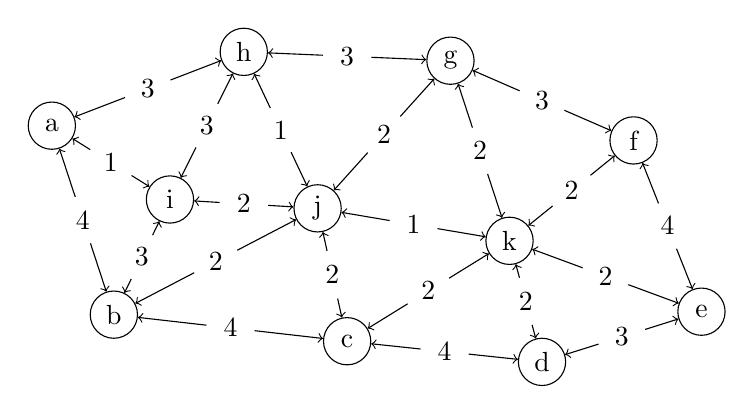
\begin{tikzpicture}[scale=0.750]
        \node[circle, draw, minimum size=0.6cm, inner sep=0pt] at (0.5* 0.0, 0.5* 8.5)  (a)    {a};
        \node[circle, draw, minimum size=0.6cm, inner sep=0pt] at (0.5* 2.1, 0.5* 2.1)  (b)    {b};
        \node[circle, draw, minimum size=0.6cm, inner sep=0pt] at (0.5* 10.0, 0.5* 1.2)  (c)    {c};
        \node[circle, draw, minimum size=0.6cm, inner sep=0pt] at (0.5* 16.6, 0.5* 0.5)  (d)    {d};
        \node[circle, draw, minimum size=0.6cm, inner sep=0pt] at (0.5* 22.0, 0.5* 2.2)  (e)    {e};
        \node[circle, draw, minimum size=0.6cm, inner sep=0pt] at (0.5* 19.7, 0.5* 8.0)  (f)    {f};
        \node[circle, draw, minimum size=0.6cm, inner sep=0pt] at (0.5* 13.5, 0.5* 10.7)  (g)    {g};
        \node[circle, draw, minimum size=0.6cm, inner sep=0pt] at (0.5* 6.5, 0.5* 11.0)  (h)    {h};
        \node[circle, draw, minimum size=0.6cm, inner sep=0pt] at (0.5* 4.0, 0.5* 6.0)  (i)    {i};
        \node[circle, draw, minimum size=0.6cm, inner sep=0pt] at (0.5* 9.0, 0.5* 5.7)  (j)    {j};
        \node[circle, draw, minimum size=0.6cm, inner sep=0pt] at (0.5* 15.5, 0.5* 4.6)  (k)    {k};

        \draw[<->]  (a) edge node[circle, fill=white] {4} (b);
        \draw[<->]  (a) edge node[circle, fill=white] {3} (h);
        \draw[<->]  (a) edge node[circle, fill=white] {1} (i);

        \draw[<->]  (b) edge node[circle, fill=white] {4} (c);
        \draw[<->]  (b) edge node[circle, fill=white] {3} (i);
        \draw[<->]  (b) edge node[circle, fill=white] {2} (j);

        \draw[<->]  (c) edge node[circle, fill=white] {4} (d);
        \draw[<->]  (c) edge node[circle, fill=white] {2} (j);
        \draw[<->]  (c) edge node[circle, fill=white] {2} (k);

        \draw[<->]  (d) edge node[circle, fill=white] {3} (e);
        \draw[<->]  (d) edge node[circle, fill=white] {2} (k);

        \draw[<->]  (e) edge node[circle, fill=white] {4} (f);
        \draw[<->]  (e) edge node[circle, fill=white] {2} (k);

        \draw[<->]  (f) edge node[circle, fill=white] {3} (g);
        \draw[<->]  (f) edge node[circle, fill=white] {2} (k);

        \draw[<->]  (g) edge node[circle, fill=white] {3} (h);
        \draw[<->]  (g) edge node[circle, fill=white] {2} (j);
        \draw[<->]  (g) edge node[circle, fill=white] {2} (k);

        \draw[<->]  (h) edge node[circle, fill=white] {3} (i);
        \draw[<->]  (h) edge node[circle, fill=white] {1} (j);

        \draw[<->]  (i) edge node[circle, fill=white] {2} (j);

        \draw[<->]  (j) edge node[circle, fill=white] {1} (k);
      \end{tikzpicture}
    }
    \caption{Vor der Kontraktion}
  \end{subfigure}
  \hfill
  \begin{subfigure}[b]{0.49\textwidth}
    \centering
    \resizebox{\textwidth}{!}{% <------ Don't forget this %
      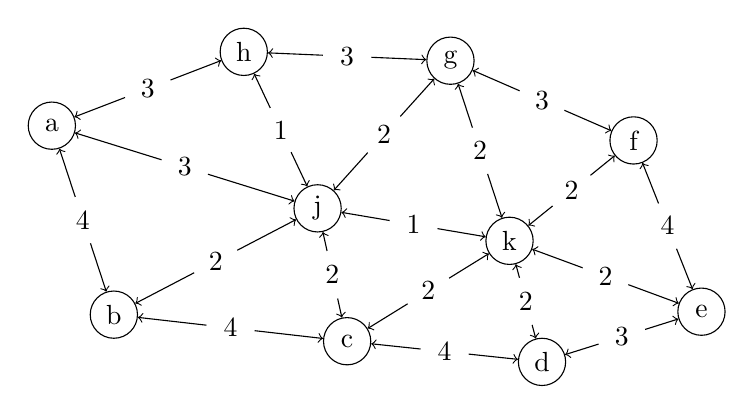
\begin{tikzpicture}[scale=0.750]
        % Nodes
        \node[circle, draw, minimum size=0.6cm, inner sep=0pt] at (0.5* 0.0, 0.5* 8.5)  (a)    {a};
        \node[circle, draw, minimum size=0.6cm, inner sep=0pt] at (0.5* 2.1, 0.5* 2.1)  (b)    {b};
        \node[circle, draw, minimum size=0.6cm, inner sep=0pt] at (0.5* 10.0, 0.5* 1.2)  (c)    {c};
        \node[circle, draw, minimum size=0.6cm, inner sep=0pt] at (0.5* 16.6, 0.5* 0.5)  (d)    {d};
        \node[circle, draw, minimum size=0.6cm, inner sep=0pt] at (0.5* 22.0, 0.5* 2.2)  (e)    {e};
        \node[circle, draw, minimum size=0.6cm, inner sep=0pt] at (0.5* 19.7, 0.5* 8.0)  (f)    {f};
        \node[circle, draw, minimum size=0.6cm, inner sep=0pt] at (0.5* 13.5, 0.5* 10.7)  (g)    {g};
        \node[circle, draw, minimum size=0.6cm, inner sep=0pt] at (0.5* 6.5, 0.5* 11.0)  (h)    {h};
        % \node[circle, draw, minimum size=0.6cm, inner sep=0pt] at (0.5* 4.0, 0.5* 6.0)  (i)    {i};
        \node[circle, draw, minimum size=0.6cm, inner sep=0pt] at (0.5* 9.0, 0.5* 5.7)  (j)    {j};
        \node[circle, draw, minimum size=0.6cm, inner sep=0pt] at (0.5* 15.5, 0.5* 4.6)  (k)    {k};

        \draw[<->]  (a) edge node[circle, fill=white] {4} (b);
        \draw[<->]  (a) edge node[circle, fill=white] {3} (h);
        \draw[<->]  (a) edge node[circle, fill=white] {3} (j);

        \draw[<->]  (b) edge node[circle, fill=white] {4} (c);
        \draw[<->]  (b) edge node[circle, fill=white] {2} (j);

        \draw[<->]  (c) edge node[circle, fill=white] {4} (d);
        \draw[<->]  (c) edge node[circle, fill=white] {2} (j);
        \draw[<->]  (c) edge node[circle, fill=white] {2} (k);

        \draw[<->]  (d) edge node[circle, fill=white] {3} (e);
        \draw[<->]  (d) edge node[circle, fill=white] {2} (k);

        \draw[<->]  (e) edge node[circle, fill=white] {4} (f);
        \draw[<->]  (e) edge node[circle, fill=white] {2} (k);

        \draw[<->]  (f) edge node[circle, fill=white] {3} (g);
        \draw[<->]  (f) edge node[circle, fill=white] {2} (k);

        \draw[<->]  (g) edge node[circle, fill=white] {3} (h);
        \draw[<->]  (g) edge node[circle, fill=white] {2} (j);
        \draw[<->]  (g) edge node[circle, fill=white] {2} (k);

        \draw[<->]  (h) edge node[circle, fill=white] {1} (j);

        \draw[<->]  (j) edge node[circle, fill=white] {1} (k);
      \end{tikzpicture}
    }
    \caption{Nach der Kontraktion}
  \end{subfigure}
  \caption{Kontraktion von $i$}
  \label{graphs:fig:example_contraction}
\end{figure}

Häufig wird die Kontraktionsbedingung abgeschwächt, indem dann eine Kante eingefügt wird, wenn der zu kontrahierende Knoten auf \emph{einem} kürzesten Pfad liegt.
Dazu kann eine normale Dijkstra-Suche verwendet werden: Ist die Länge einer potenziellen Abkürzung optimal, dann wird sie eingefügt.
Da die Suche, die $(v, w)$ nicht durchläuft, den gesamten Graphen absucht, wenn $(u, v, w)$ der einzige $u$-$w$-Pfad ist, kann die normale Dijkstra-Suche im Vergleich zur Modifizierten deutlich effektiver sein.
Weiter kann die Anzahl der Hops der Suche begrenzt werden.
Dadurch können jedoch auch Kanten eingefügt werden, die nicht unbedingt für die Erhaltung der Abstände erforderlich sind.

\subsection{Graphen-Kontraktion}

Um die Datenstruktur für die Beantwortung von Anfragen, den \emph{Contracted-Graph}, zu erstellen, müssen alle Knoten eines Graphen kontrahiert werden. Die Kanten, die in jedem Schritt entfernt werden, werden dabei gesammelt.
Hierbei hat die Reihenfolge, in der das geschieht, einen großen Einfluss auf die Performance der nachfolgenden Kontraktionen und den mit der Methode erzielte Speedup.
Die Reihenfolge der Kontraktion wird durch eine \emph{vertex-to-level}-Funktion angegeben.
Sie ist bijektiv und definiert als ${vtl} \colon V \to L$ mit $L \subset \mathbb{N}$, $\abs{L} = \abs{V}$ und $\max(L) = \abs{V}$.
Der Knoten mit dem niedrigsten \emph{Level} wird dabei zuerst kontrahiert.
Ihre Umkehrfunktion wird \emph{level-to-vertex}-Funktion genannt.

\begin{definition}[Contracted-Graph]
  Sei $G = (V, E)$ und $E'$ die durch die vollständige Kontraktion von $G$ erhaltenen Kanten mit der dazugehörigen vertex-to-level-Funktion ${vtl}$.

  Ein Contracted-Graph ist dann ein Tupel $C = (G_u, G_d)$. Der \emph{Upward-Graph} ist dabei $G_u = (V, E_u)$ mit $E_u = \{ (t, h) \mid (t, h) \in E' \colon {vtl}(h) > {vtl}(t) \}$, der \emph{Downward-Graph} ist $G_d = (V, E_d)$ mit $E_d = \{ (h, t) \mid (t, h) \in E' \colon {vtl}(h) < {vtl}(t) \}$.
\end{definition}

Der Name Upward-Graph leitet sich daraus ab, dass die Suche innerhalb dieses Graphen bezogen auf die Level ausschließlich \emph{aufwärts} erfolgt.
Geisberger et al. \cite{geisberger2008contraction} transponieren die Kanten des Downward-Graphen nicht, daher geht ihre Suche \emph{abwärts}.
Die Transposition der Kanten ist hierbei nur eine Methode, damit auf dem Downward-Graphen wie auf dem Upward-Graphen \emph{vorwärts} gesucht wird.

Der entstandene Graph ist azyklisch, da er nur Kanten enthält, deren Kopf ein größeres Level als der dazugehörige Fuß hat.
Die Anzahl der in einer Breitensuche gefundenen Knoten ist geringer als im Ursprungsgraphen.
Diese Eigenschaften sorgen dafür, dass eine Suche in einem Upward-Graph kostengünstiger sein kann.
Die kürzesten Pfade, die im Upward-Graph gefunden worden, bilden eine obere Schranke für die tatsächlich kürzesten Pfade in $G$, in einigen Fällen können sie jedoch länger sein.
\autoref{graphs:fig:counterexample_optimal_Upward} zeigt ein Beispiel hierzu.
Die Knoten sind in der Reihenfolge $c$, $d$, $a$, $b$ kontrahiert worden, wodurch der dazugehörige Upward-Graph entsteht.
Der optimale $c$-$a$-Pfad in $G$ hat die Distanz zwei, in $G_u$ hat er jedoch die Distanz drei.

\begin{figure}[ht]
  \centering
  \begin{subfigure}[b]{0.49\textwidth}
    \centering
    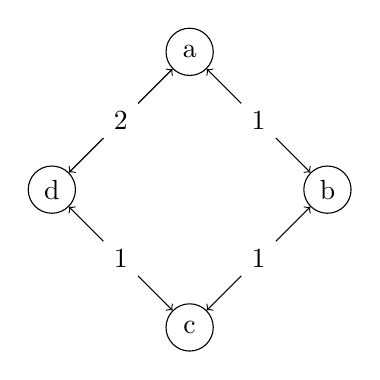
\begin{tikzpicture}
      \node[circle, draw, minimum size=0.6cm, inner sep=0pt] at (1.75*1.0, 1.75*2.0)  (a)    {a};
      \node[circle, draw, minimum size=0.6cm, inner sep=0pt] at (1.75*2.0, 1.75*1.0)  (b)    {b};
      \node[circle, draw, minimum size=0.6cm, inner sep=0pt] at (1.75*1.0, 1.75*0.0)  (c)    {c};
      \node[circle, draw, minimum size=0.6cm, inner sep=0pt] at (1.75*0.0, 1.75*1.0)  (d)    {d};

      \draw[<->]  (a) edge node[circle, fill=white] {1} (b);
      \draw[<->]  (b) edge node[circle, fill=white] {1} (c);
      \draw[<->]  (c) edge node[circle, fill=white] {1} (d);
      \draw[<->]  (d) edge node[circle, fill=white] {2} (a);
    \end{tikzpicture}
    \caption{Graph $G$}
  \end{subfigure}
  \hfill
  \begin{subfigure}[b]{0.49\textwidth}
    \centering
    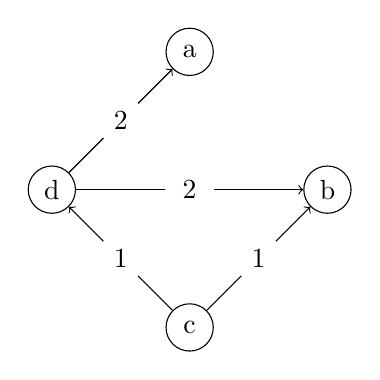
\begin{tikzpicture}
      \node[circle, draw, minimum size=0.6cm, inner sep=0pt] at (1.75*1.0, 1.75*2.0)  (a)    {a};
      \node[circle, draw, minimum size=0.6cm, inner sep=0pt] at (1.75*2.0, 1.75*1.0)  (b)    {b};
      \node[circle, draw, minimum size=0.6cm, inner sep=0pt] at (1.75*1.0, 1.75*0.0)  (c)    {c};
      \node[circle, draw, minimum size=0.6cm, inner sep=0pt] at (1.75*0.0, 1.75*1.0)  (d)    {d};

      \draw[->]  (c) edge node[circle, fill=white] {1} (b);
      \draw[->]  (c) edge node[circle, fill=white] {1} (d);
      \draw[->]  (d) edge node[circle, fill=white] {2} (b);
      \draw[->]  (d) edge node[circle, fill=white] {2} (a);
    \end{tikzpicture}
    \caption{Upward-Graph $G_u$ zu $G$}
  \end{subfigure}
  \caption{Gegenbeispiel optimale Kosten im $G_u$}
  \label{graphs:fig:counterexample_optimal_Upward}
\end{figure}

\subsection{Anfragen}

Die Suche eines kürzesten Pfades von $a$ nach $e$ auf dem Beispielgraphen gestaltet sich nun wie folgt:
Auf $G_u$ wird eine Dijkstra-Suche von $a$ und auf $G_d$ eine Dijkstra-Suche von $e$ durchgeführt.
Aus den von beiden Dijkstra-Suchen besuchten Knoten wird nun derjenige ausgewählt, der die niedrigste Summe beider Distanzen aufweist.
\autoref{fig:ch:beispiel_suche} zeigt den auf diese Weise gefundenen Pfad im Beispielgraphen von $a$ nach $e$.
Die Level der Knoten auf dem Pfad steigen von beiden Seiten an, bis sie den Treffpunktknoten $j$ erreichen.
Hierbei ist die Kante $(a, j)$ eine Abkürzung, sie kürzt $i$ ab, was durch die gestrichelten Pfeile angedeutet wird.

\begin{figure}[ht]
  \centering
  \begin{tikzpicture}
    \node[circle, draw] at (0 * 1.5, -2 * 0.75)  (a)    {a};
    \node[circle, draw] at (1 * 1.5, -4 * 0.75)  (i)    {i};
    \node[circle, draw] at (2 * 1.5, -0 * 0.75)  (j)    {j};
    \node[circle, draw] at (3 * 1.5, -1 * 0.75)  (k)    {k};
    \node[circle, draw] at (4 * 1.5, -3 * 0.75)  (e)    {e};

    % draw axis
    \draw[->] (-1, -4 * 0.75) -- (-1, 0) node[above] {Level};

    \draw[->]  (a) -- (j);
    \draw[->]  (e) -- (k);
    \draw[->]  (k) -- (j);

    \draw[->, dotted]  (a) -- (i);
    \draw[->, dotted]  (i) -- (j);

  \end{tikzpicture}
  \caption{Beispiel einer Suche im Contracted-Graph}
  \label{fig:ch:beispiel_suche}
\end{figure}

Algorithmus \ref{ch:query_simple} definiert dies formal.
Wie bei einer bidirektionalen Dijkstra-Suche wird der Pfad, sofern existent, aus den Teilpfaden beider Suchen erstellt.
Diese haben die Form $(u, \dotsc, t)$ beziehungsweise $(v, \dotsc, t)$.
Um einen gültigen Pfad zu erstellen, muss $t$ aus einem dieser Teilpfade entfernt und der Pfad des Downward-Graphen umgekehrt werden.
Anschließend können beide Pfade konkateniert werden, somit entsteht ein Pfad auf $C$ der Form $(u, \dotsc, t, \dotsc, v)$.
Dieser muss jedoch nicht unbedingt ein gültiger Pfad auf $G$ sein, da er noch Abkürzungen enthalten kann.
In \autoref{ch:subsection:pfad_gewinnung} wird darauf eingegangen, wie diese entfernt werden können.

\begin{algorithm}[ht]
  \caption{Contraction Hierarchies Query}
  \begin{algorithmic}[1]
    \Require Upward-Graph $G_u = (V, E_u)$, Downward-Graph $G_d = (V, E_d)$, Startknoten $s \in V$, Zielknoten $t \in V$
    \Ensure Treffpunktknoten $m \in V \cup \{ {none} \}$, ${dist}_u$, ${pre}_u$, ${dist}_d$, ${pre}_d$
    \State ${dist}_u$, ${pre}_u$ $\leftarrow$ Dijkstra$(G_u, s)$
    \State ${dist}_d$, ${pre}_d$ $\leftarrow$ Dijkstra$(G_d, t)$

    \State
    \State $m \leftarrow {none}$
    \State $d \leftarrow \infty$
    \State
    \ForAll {$v \in V$}
    \If {${dist}_u(v) + {dist}_d(v) < d$}
    \State $m \leftarrow v$
    \State $d \leftarrow {dist}_u(v) + {dist}_d(v)$
    \EndIf
    \EndFor

    \State
    \State \Return $m$, ${dist}_u$, ${pre}_u$, ${dist}_d$, ${pre}_d$
  \end{algorithmic}
  \label{ch:query_simple}
\end{algorithm}

Die Korrektheit des Algorithmus ist nicht sofort ersichtlich, da nicht alle besuchten Knoten eine optimale Distanz haben und nur ein Teil aller Knoten besucht wird.
Der Beweis hierfür betrachtet einen kürzesten Pfad auf $G$ und argumentiert, warum dieser gefunden wird:


\begin{beweis}[Korrektheit der Contracted-Graph-Anfrage]\label{ch:proof:correct}
  Der Upward-Graph $G_u$ und der Downward-Graph $G_d$ enthalten nur Kanten, die mindestens so lang sind wie der Abstand in $G$.
  Daher kann ein $s$-$t$-Pfad in $C$ nur dann gefunden werden, wenn auch in $G$ ein solcher Pfad existiert.

  Es ist zu zeigen, dass eine Suche auf $C$ den Abstand in $G$ liefert.
  Sei $\text{sp}_G(s, t)$ ein kürzester Pfad auf $G$, der unter allen kürzesten Pfaden den Knoten $m$ mit dem höchsten Level enthält.
  Aus diesem Pfad $(s, \dotsc, t)$ werden zwei Teilpfade konstruiert: $(s, \dotsc, m)$ und $(t, \dotsc, m)$.

  Betrachte den Teilpfad $(s, \dotsc, m)$ mit der Hop-Länge $n_u$.
  Entferne aus diesem Pfad alle Knoten zwischen $s$ und $m$, die ein kleineres Level als ihre Vorgänger haben.
  Dieser Vorgang wird so oft wiederholt, bis keine weiteren Knoten mehr entfernt werden können.

  Der resultierende Pfad besteht aus überlappenden Tupeln der Form $(v_{i}, v_{i + 1})$.
  Für diese gilt $\text{vtl}(v_i) < \text{vtl}(v_{i + 1})$, da sich der Pfad im Upward-Graph befindet.
  Die Knoten-Kontraktion erhält die Abstände der verbleibenden Knoten.
  Zum Zeitpunkt der Kontraktion von $v_i$ existierte also ein optimaler Pfad von $v_i$ zu $v_{i + 1}$.
  Alle Knoten, die ursprünglich zwischen ihnen lagen und entfernt wurden, haben ein kleineres Level als $v_i$ und waren zum Zeitpunkt der Kontraktion von $v_i$ bereits kontrahiert.
  Daher existierte vor der Kontraktion von $v_i$ eine direkte Kante zu $v_{i + 1}$, die gesammelt und zum Aufbau des Upward-Graphen verwendet wurde.
  Somit wird $v_{i + 1}$ von $v_i$ aus erreicht.
  Da dies für alle überlappenden Tupel gilt, wird $m$ von $s$ aus mit optimalem Abstand erreicht.

  Analog wird für den Teilpfad $(t, \dotsc, m)$ im Downward-Graph argumentiert.
  \qed
\end{beweis}

\subsection{Erstellung des Pfades}\label{ch:subsection:pfad_gewinnung}

Der in $C$ gefundene Pfad kann noch Abkürzungen enthalten.
Damit der Pfad auch auf $G$ gültig ist, müssen diese ersetzt werden.
Hierfür ist eine Funktion notwendig, welche diese ersetzt.

Eine solche Abkürzungsfunktion kann etwa durch eine HashMap implementiert werden.
Da die ${vtl}$-Funktion bijektiv ist, gilt für alle Knoten $u, v \in V$, $u \neq v$ immer entweder ${vtl}(u) < {vtl}(v)$ oder ${vtl}(u) > {vtl}(v)$.
Daher reicht es für die Ersetzung der Abkürzungen in Pfaden in $C$ \emph{eine} HashMap zu benutzen, da keine Kollisionen zwischen Abkürzungen des Upward- und des Downward-Graphen entstehen können.

\begin{figure}[ht]
  \centering
  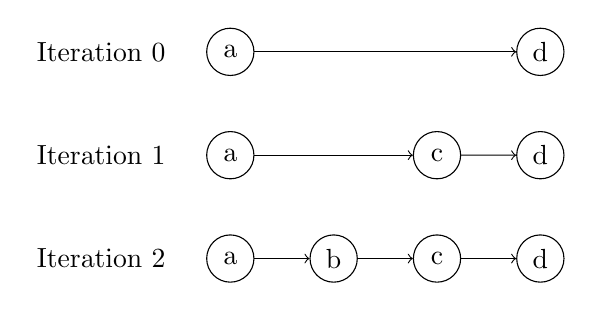
\begin{tikzpicture}[scale=0.75]
    \node[align=left] at (1.75*-1.25,1.75*2) {Iteration 0};
    \node[circle, draw, minimum size=0.6cm, inner sep=0pt] at (1.75*0.0, 1.75*2.0)  (a_0)    {a};
    \node[circle, draw, minimum size=0.6cm, inner sep=0pt] at (1.75*3.0, 1.75*2.0)  (d_0)    {d};
    \draw[->]  (a_0) edge node {} (d_0);

    \node[align=left] at (1.75*-1.25,1.75*1) {Iteration 1};
    \node[circle, draw, minimum size=0.6cm, inner sep=0pt] at (1.75*0.0, 1.75*1.0)  (a_1)    {a};
    \node[circle, draw, minimum size=0.6cm, inner sep=0pt] at (1.75*2.0, 1.75*1.0)  (c_1)    {c};
    \node[circle, draw, minimum size=0.6cm, inner sep=0pt] at (1.75*3.0, 1.75*1.0)  (d_1)    {d};
    \draw[->]  (a_1) edge node {} (c_1);
    \draw[->]  (c_1) edge node {} (d_1);

    \node[align=left] at (1.75*-1.25,1.75*0) {Iteration 2};
    \node[circle, draw, minimum size=0.6cm, inner sep=0pt] at (1.75*0.0, 1.75*0.0)  (a_2)    {a};
    \node[circle, draw, minimum size=0.6cm, inner sep=0pt] at (1.75*1.0, 1.75*0.0)  (b_2)    {b};
    \node[circle, draw, minimum size=0.6cm, inner sep=0pt] at (1.75*2.0, 1.75*0.0)  (c_2)    {c};
    \node[circle, draw, minimum size=0.6cm, inner sep=0pt] at (1.75*3.0, 1.75*0.0)  (d_2)    {d};
    \draw[->]  (a_2) edge node {} (b_2);
    \draw[->]  (b_2) edge node {} (c_2);
    \draw[->]  (c_2) edge node {} (d_2);
  \end{tikzpicture}
  \caption{Beispiel des iterativen Ersetzen von Abkürzungen}
\end{figure}

Um diese Funktion zu erhalten, müssen die Abkürzungen, welche beim Kontrahieren des Graphen eingefügt werden, und die dabei übersprungenen Knoten gesammelt werden.
Einen möglichen Algorithmus, der Abkürzungen in einem Pfad ersetzt, ist in Algorithmus \ref{ch:alg:shortcut_replacement} zu sehen.
Dieser betrachtet den Pfad mit Abkürzungen als Stapel und bearbeitet jeweils nur die beiden obersten Knoten, weil das Einfügen an einer bestimmten Stelle in ein Array rechenintensiv ist.

\begin{algorithm}[ht]
  \caption{Shortcut Replacement}
  \begin{algorithmic}[1]
    \Require Pfad $p$ mit Abkürzungen, Abkürzungsfunktion $S \colon V \times V \to V \cup \{ {none} \}$
    \Ensure Pfad $p'$ ohne Shortcuts

    \If {$\text{len}(p) == 1$}
    \State \Return $p$
    \EndIf
    \State

    \State $p' \leftarrow ()$
    \State

    \While {$\text{len}(p) >= 2$}
    \State $w \leftarrow \text{pop}(p)$
    \State $u \leftarrow \text{pop}(p)$
    \State $v \leftarrow S((u, w))$
    \State

    \If {$v \neq none$}
    \State $\text{push}(p, u)$
    \State $\text{push}(p, v)$
    \State $\text{push}(p, w)$
    \Else
    \State $\text{push}(p, u)$
    \State $\text{push}(p', w)$
    \EndIf
    \EndWhile

    \State
    \State $p' \leftarrow \text{reversed}(p')$

    \State
    \State \Return $p'$
  \end{algorithmic}
  \label{ch:alg:shortcut_replacement}
\end{algorithm}

\subsection{Early Stop}

Algorithmus \ref{ch:query_simple} hat primär theoretische Bedeutung.
Implementierungen ähneln der bidirektionalen Dijkstra-Suche, dabei werden abwechselnd Knoten der Upward-Suche und der Downward-Suche expandiert.
Die Expansion einer Suchrichtung wird gestoppt, wenn die kleinste Distanz der Vorwärtswarteschlange größer als die bisherige kleinste Treffpunkt-Distanz ist.
Sobald beide Suchen gestoppt wurden, ist der kürzeste Pfad, falls vorhanden, gefunden.

\subsection{stall-on-demand}

Wie \autoref{graphs:fig:counterexample_optimal_Upward} zeigt, sind manche der im Upward- und Downward-Graphen gefundenen Distanzen nicht optimal.
Für das Finden eines kürzesten Pfades sind jedoch nur die Knoten interessant, deren Distanz optimal ist.
Mit der von Schultes und Sanders \cite{schultes2007dynamic} vorgestellten Methode \emph{stall-on-demand} ist es möglich, den Suchraum der beiden Teilsuchen einzuschränken.
Hierfür wird die Expansion eines Knotens abgebrochen, wenn er über eine Kante des jeweils anderen Graphen günstiger erreicht werden kann.

\begin{definition}[stall-on-demand]
  Sei $C = (G_u, G_d)$ ein Contracted-Graph mit $G_u = (V, E_u)$ und $G_d = (V, E_d)$.
  Der Knoten $u \in V$ hat keine optimale Distanz in der Dijkstra-Suche von $s$ in $G_u$, wenn es zum Zeitpunkt seiner Expansion eine Kante $(u, v, d) \in E_d$, $v \in V$, $d \in \mathbb{R}$ gibt mit ${dist}(v) + d < {dist}(u)$.
  Die Expansion von $u$ kann dann abgebrochen werden, die aus $u$ ausgehenden Kanten müssen nicht betrachtet werden.
  Gleiches gilt analog für $G_d$.
\end{definition}

Veranschaulicht wird dies an dem Beispiel in \autoref{fig:ch:stall_example}, das die Suche des Upward-Graphen betrachtet.
Die blauen Kanten repräsentieren Kanten der Upward-Suche, während die rote Kante eine von $u$ ausgehende Downward-Kante darstellt.
Bisher wurde $v$ in der Upward-Suche mit einer Distanz von eins expandiert, im nächsten Schritt soll $u$ expandiert werden.
Der Knoten $u$ hat die Distanz drei in der Upward-Suche, kann jedoch über die Upward-Kante mit einer Distanz von zwei erreicht werden.
Also ist die Distanz drei nicht optimal, und von $u$ ausgehenden Kanten müssen nicht betrachtet werden.

\begin{figure}
  \centering
  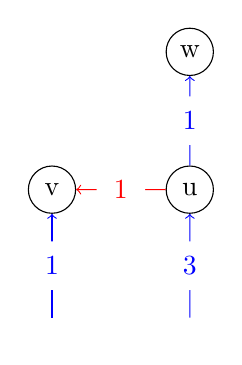
\begin{tikzpicture}[scale=1.75]
    \node[circle, draw, minimum size=0.6cm, inner sep=0pt] at (0, 2)  (v)    {v};
    \node[circle, draw, minimum size=0.6cm, inner sep=0pt] at (1, 2)  (u)    {u};
    \node[circle, draw, minimum size=0.6cm, inner sep=0pt] at (1, 3)  (w)    {w};

    \node[] at (0, 1)  (uv)    {};
    \node[] at (1, 1)  (uu)    {};

    \draw[->,blue]  (u) edge node[circle, fill=white] {1} (w);

    \draw[->,red]  (u) edge node[circle, fill=white] {1} (v);

    \draw[->,blue]  (uv) edge node[circle, fill=white] {1} (v);
    \draw[->,blue]  (uu) edge node[circle, fill=white] {3} (u);
  \end{tikzpicture}
  \caption{Beispiel stall-on-demand}
  \label{fig:ch:stall_example}
\end{figure}

\subsection{Erstellung}

Ein Contracted-Graph entsteht durch die vollständige Kontraktion eines Graphen.
Die Reihenfolge, in der die Knoten kontrahiert werden, kann im Voraus festgelegt werden, oder der jeweils \emph{unwichtigste} Knoten wird kontrahiert.
Der Prozess der Erstellung kann nach mehreren Kriterien bewertet werden, so kann die Geschwindigkeit der Erstellung, die Geschwindigkeit der Anfragen oder die Anzahl der bei der Kontraktion hinzugefügten Abkürzungen minimiert werden.

\subsubsection{Top-Down}
Bei der Top-Down-Kontraktion ist die level-to-vertex-Funktion ${ltv}$ vorgegeben.
Die Knoten werden in der Reihenfolge ihres Levels kontrahiert, wobei mit dem niedrigsten Level begonnen wird.
Diese Herangehensweise bietet die Möglichkeit eine optimale Reihenfolge anzuwenden, wobei die für hinreichend große Graphen nur schwer bestimmbar ist.

Knoten mit vielen Nachbarn können potenziell viele neue Kanten erzeugen, weshalb sie bei der \emph{Sortierung nach Grad} erst später kontrahiert werden, um dies zu verhindern.

Die Knoten können auch über ein Hitting-Set sortiert werden:
Hierbei wird auf Grundlage einer möglichst großen Anzahl von Pfaden ein Hitting-Set gebildet.
Die Knoten des Hitting-Sets werden dann nach der Anzahl ihrer Hits sortiert.
Den Knoten, die nicht Teil des Hitting-Sets sind, werden anschließend die unteren Level zugewiesen, wobei diese wiederum nach einer Metrik wie etwa dem Grad sortiert werden können.

\subsubsection{Bottom-Up}

Bei der Bottom-Up-Kontraktion wird die vertex-to-level-Funktion ${vtl}$ während der Kontraktion erstellt.
Dabei wird mithilfe einer Heuristik der jeweils \emph{unwichtigste} Knoten aus einer Prioritätswarteschlange ausgewählt und kontrahiert.
Ein unwichtiger Knoten hat einen niedrigen Heuristikwert.
Die in der Praxis am häufigsten verwendeten Heuristiken beinhalten die \emph{Kanten-Differenz}, berücksichtigen jedoch häufig auch weitere Informationen.

Die Kanten-Differenz gibt an, wie sich die Anzahl der Kanten im gesamten Graphen durch die Kontraktion eines Knotens verändert.
Sie wird berechnet, indem die Anzahl der neu hinzugefügten Kanten von der Anzahl der entfernten Kanten subtrahiert wird, wobei die Kontraktion des Knotens \emph{simuliert} wird.
Die Kontraktion eines Knotens kann die Heuristikwerte anderer Knoten beeinflussen.
Um sicherzustellen, dass stets der Knoten mit dem niedrigsten Heuristikwert ausgewählt wird, müssten nach jeder Kontraktion alle Heuristikwerte neu berechnet werden.
Da dies jedoch in der Praxis zu teuer ist, haben sich zwei Methoden als effektiv erwiesen:

Beim \emph{Lazy-Popping} wird angenommen, dass ein Knoten nur an Wichtigkeit gewinnen kann.
Aus der Warteschlange wird ein Knoten entnommen und geprüft, ob sein Heuristikwert gestiegen ist.
Falls er gestiegen ist, wird er zurück in die Warteschlange geschoben, andernfalls wird er kontrahiert.
Dies wird wiederholt, bis ein Knoten gefunden wird, dessen Heuristikwert unverändert geblieben ist.
Beim \emph{Neighbor-Update} werden nach der Kontraktion eines Knotens die Heuristikwerte der benachbarten Knoten aktualisiert.

Um die zu einem Contracted-Graph gehörende Abkürzungsfunktion zu erhalten, muss während der Kontraktion des Graphen eine Liste der Abkürzungen erstellt werden.
Wenn die im vorherigen Abschnitt erwähnte abgeschwächte Bedingung verwendet wird, muss sichergestellt werden, dass sich die Abkürzungen zweier Knoten während der Kontraktion mehrmals ändern können.
Dabei darf nur die letzte und beste Abkürzung gespeichert werden.

\section{Hierarchical Hub Labeling}\label{chapter:hl}

Die Contracted-Graph-Anfrage ohne Stopbedingung baut jeweils den vollständigen Suchbaum für den Start- und Zielknoten auf und sucht aus den expandierten Knoten beider Suchen den Knoten mit der geringsten Summe der Distanzen in beiden Suchen.
Die Idee hinter dem Labeling besteht darin, den Suchbaum des Upward- bzw. Downward-Graphen zu speichern, sodass eine $s$-$t$-Anfrage nur noch den Vergleich zweier Labels erfordert.
In der von \cite{abraham2011hub} vorgestellten Terminologie wird das Label des Upward-Graphen \emph{Forward-Label} und das des Downward-Graphen \emph{Backward-Label} genannt.
Ein kürzester Pfad wird bestimmt, indem der Knoten mit der geringsten Summe der Distanzen im Forward- und Backward-Label gefunden wird.

\begin{definition}[Hub Graph]
  Sei $G = (V, E)$.
  Ein \emph{Hub Graph} ist definiert als $H = (L_f, L_b)$ und es gilt:
  Die Forward-Label-Funktion $L_f \colon V \to V \times \mathbb{R}^+_0$ weist jedem Knoten ein Forward-Label zu.
  Sei $L_f(u)$ das Forward-Label des Knotens $u \in V$, dann gibt es für jeden Knoten $v \in V$ höchstens einen Eintrag $(v, d) \in L_f(u)$ und es gilt $d \geq {spd}_G(u, v)$.
  Ein Backward-Label entspricht dem Forward-Label des transponierten Graphen $G^T$.

  Forward- und Backward-Labels erfüllen zusammen die \emph{Abdeckungseigenschaft}:
  Für jedes Knotenpaar $s, t \in V$, für das ein kürzester $s$-$t$-Pfad existiert, gibt es einen Knoten $m \in V$ mit $(m, d_f) \in L_f(s)$, $(m, d_r) \in L_r(t)$ und $d_f + d_r = {spd}_G(s, t)$.
\end{definition}

Die Definition der Labels ähnelt dem Beweis der Korrektheit der Contracted-Graph-Anfrage, bei dem ebenfalls mit einem Treffpunktknoten $m$ argumentiert wird.
Aus einem Contracted-Graphen lässt sich ein Hub-Graph konstruieren, indem die Suchbäume des Upward-Graphen als Forward-Labels und die des Downward-Graphen als Backward-Labels betrachtet werden, da sich die Suchbäume im Knoten mit dem höchsten Level und dem optimalen Abstand treffen.

Die Erstellung der Labels kann auf zwei Arten erfolgen: durch eine Dijkstra-Suche im Upward- bzw. Downward-Graphen für jeden Knoten oder durch \emph{Merging}.
Die so erstellten Labels sind \emph{hierarchisch}:
Es existiert eine Reihenfolge der Knoten (definiert durch die vertex-to-level-Funktion), sodass das Forward- und Backward-Label eines Knotens $u$ nur Knoten $h$ mit höherem Level enthält.
Es gibt auch Labels, die diese hierarchische Eigenschaft nicht erfüllen, solche Labels können für bestimmte Graphen erheblich kleiner sein als hierarchische Labels \cite{goldberg2013separating}.

\subsubsection{Anfrage}

Sei $H = (L_f, L_b)$ ein Hub-Graph.
Algorithmus \ref{hl:alg:query} zeigt, wie wenige Schritte notwendig sind, um einen Abstand in $H$ zu finden: Dafür ist nur noch das Finden des Knotens mit der geringsten Summe der Distanzen erforderlich.
Da die Labels den Suchbäumen der Upward- und Downward-Suche entsprechen, ist die Korrektheit der Hub-Graph-Anfrage durch die Korrektheit der Contracted-Graph-Anfrage gegeben.

\begin{algorithm}[ht]
  \caption{Hub-Label-Anfrage}
  \begin{algorithmic}[1]
    \Require Forward-Label-Funktion $L_f$, Backward-Label-Funktion $L_b$, Startknoten $s \in V$, Zielknoten $t \in V$
    \Ensure Treffpunktknoten $m \in V \cup \{ {none} \}$, ${dist}_u$
    \State $l_s \leftarrow L_f (s)$
    \State $l_t \leftarrow L_b (t)$

    \State
    \State $m \leftarrow {none}$
    \State $d \leftarrow \infty$

    \ForAll {$v \in V \colon (v, d_f) \in l_s \land (v, d_r) \in l_t$}
    \If {$d_f + d_r < d$}
    \State $d \leftarrow d_f + d_r$
    \State $m \leftarrow v$
    \EndIf
    \EndFor

    \State
    \State \Return $m$, $d$
  \end{algorithmic}
  \label{hl:alg:query}
\end{algorithm}

\subsection{Pfaderstellung}

Nachdem ein Treffpunktknoten $m$ gefunden wurde, sind noch zusätzliche Informationen notwendig, um einen Pfad in $G$ erstellen zu können, denn zuerst muss ein Pfad in $C$ erstellt werden, und anschließend müssen die Abkürzungen ersetzt werden.
Dazu muss für jeden Knoten in einem Label der Vorgänger, falls vorhanden, bekannt sein.
Dafür wird die Definition des Labels von einer Teilmenge von $V \times \mathbb{R}$ erweitert auf eine Teilmenge von $V \times \mathbb{R} \times (V \cup \{ none \}) $.
Der zusätzliche Eintrag speichert hierbei den Vorgänger.
Um den Pfad zu erstellen, beginnt man beim Treffpunktknoten und folgt den Vorgängern, bis kein Vorgänger mehr existiert.
Durch das Ersetzen der Abkürzungen, etwa mit dem Algorithmus \ref{ch:alg:shortcut_replacement}, erhält man so einen gültigen Pfad auf $G$.

\subsection{Datenstruktur}

Gibt es eine Totalordnung der Knoten, lässt sich durch eine geschickte Wahl der Datenstruktur zur Speicherung der Labels der Treffpunktknoten in linearer Zeit zur Größe der Labels finden.
Labels sind dann Listen, deren Einträge nach den Knoten sortiert sind.
Ähnlich wie bei Mergesort werden dabei die Einträge paarweise verglichen, wobei der Index des Labels mit dem jeweils kleineren Element inkrementiert wird.
Dadurch ist garantiert, dass alle Knoten, die in \emph{beiden} Labels vorhanden sind, gleichzeitig betrachtet werden.
Falls sie einen aktuell besten Treffpunktknoten bilden, kann diese Information gespeichert werden.

Um das Finden der Vorgänger effizienter zu gestalten, wird nicht der Vorgänger selbst gespeichert, sondern dessen Index im Label.
\autoref{ch:fig:label} zeigt ein Label dieser Art.

\begin{figure}[ht]
  \centering
  \begin{tabular}{@{}llllll@{}}
    \toprule
    Index           &  & 0   & 1   & 2   & 2 \\ \midrule
    Vertex          &  & $e$ & $j$ & $k$ &   \\
    Distanz         &  & 0   & 3   & 2   &   \\
    Vorgänger Index &  & -   & 2   & 0   &   \\ \bottomrule
  \end{tabular}
  \caption{Beispiel eines Labels}
  \label{ch:fig:label}
\end{figure}

\subsection{Erstellung}

Da die Labels den expandierten Knoten im Suchbaum des Upward- bzw. Downward-Graphen entsprechen, können diese naiv dadurch erstellt werden, dass für jeden Knoten der entsprechende Suchbaum mithilfe einer Dijkstra-Suche erstellt und die gefundenen Knoten sortiert werden.
Das lässt sich gut parallelisieren, jedoch ist das \emph{Merging} meist effizienter.

\subsubsection{Merging}

Für jeden Knoten des Graphen $G$ wird ein Label vorbereitet, das zu Beginn nur den Knoten selbst enthält.
Danach werden die Labels in der Reihenfolge der Level, von groß zu klein, wie folgt erstellt: Für jeden Knoten werden die ausgehenden Kanten des Downward- bzw. Upward-Graphen betrachtet.
Die Köpfe dieser Kanten haben ein höheres Level als der Knoten selbst, daher existieren ihre Labels bereits.
Sie werden gemerged, um ein neues Label zu bilden.
Ist ein Knoten mit mehreren Distanzen im Label, so wird nur der Eintrag mit der kleinsten Distanz übernommen.
Dabei entstehen gleichzeitig die benötigten Suchbäume des Upward- bzw. Downward-Graphen.

\subsubsection{Pruning}

Die erstellten Labels enthalten bisher noch Knoten mit nicht-optimaler Distanz in $G$ (siehe \autoref{graphs:fig:counterexample_optimal_Upward}), was sowohl den Speicherbedarf der Labels als auch die Anfragezeiten erhöht.
Die Einträge mit nicht-optimaler Distanz können entfernt werden, indem die erstellten Hub-Labels verwendet werden, um diese Einträge zu identifizieren.
Diese nicht-optimalen Einträge können dann aus den Labels entfernt werden.
Beim Merging kann dies auch bereits während der Erstellung geschehen, da die Labels von Knoten mit höherem Level bereits existieren.
